


%-------------------------------

\newpage

\section{Systematic Review and Modelography}{Revue Systématique et Modélographie}

\label{sec:modelography}

%-------------------------------


Tandis que les études menées précédemment proposaient de construire un horizon global de l'organisation des disciplines s'intéressant à notre question, nous proposons à présent une étude plus ciblée des caractéristiques de modèles existants. Nous proposons pour cela dans un premier temps une revue systématique, c'est à dire la construction d'un corpus plus précis répondant à certaines contraintes, suivie d'une meta-analyse, c'est à dire une tentative d'explication de certaines caractéristiques des modèles par des modèles statistiques.


%%%%%%%%%%%%%%%%%%%%
\subsection[Systematic Review][Revue Systématique]{Systematic Review and Meta-analysis}{Revue systématique et Meta-analyse}



Les revues systématiques classiques ont majoritairement lieu dans des domaines où une recherche très ciblée, même par titre d'article, fournira un certain nombre d'études étudiant quasiment la même question : typiquement en évaluation thérapeutique, où des études standardisées d'une même molécule varient uniquement par taille des effectifs et modalités statistiques (groupe de contrôle, placebo, niveau d'aveugle). Dans ce cas la construction du corpus est d'une part aisée par l'existence de bases spécialisées permettant des recherches très ciblées, et d'autre part par la possibilité de procéder à des analyses statistiques supplémentaires pour croiser les différentes études (par exemple meta-analyse par réseau, voir~\cite{rucker2012network}). Dans notre cas, l'exercice est bien plus aléatoire pour les raisons exposées dans les deux sections précédentes : les objets sont hybrides, les problématiques diverses, et les disciplines variées. Les différents points soulevés par la suite auront souvent autant de valeur thématique que de valeur méthodologique, suggérant des points cruciaux lors de la réalisation d'une telle revue systématique hybride.


Nous proposons une méthodologie hybride couplant les deux méthodologies développées précédemment avec une procédure plus classique de revue systématique. Nous souhaitons à la fois une représentativité de l'ensemble des disciplines que l'on a découvertes, mais aussi un bruit limité dans les références prises en compte pour la modélographie. Nous adoptons pour cela le protocole suivant :

% - 0.95% of edges with higher weight, with nodes in 80% quantile degree of their respective sem class.
% - take pairs (edges) and singles : 2582 kws
% - filter by hand : typically removed : Emissions, Education-cgnitive sci, teledetection, migration, social nws, lieux-pays, tourism-culture, social inequalities etc,  ; and too general : spillover e.g.  -> 115kws
% - request : can ask for 20 in that case
% - corpus : 2001 references
% - manual screening (title) 
%    * we already remove mobility studies (other scale) to limit final corpus
%    * pedestrian models
%    * traffic
%    * random stuffs
%    * design only (transport or lu independently) (≠ nw growth Tero)
%    * travel behavior : impact car ownersjip urb form, impact biofuel policies US, 
%    * ecology (habitat)
%    * technical transport
%    * pure eco (agllo eco) Anas urban spatial structure
%    * freight
%
%  -> N = 134 at this stage -> extend with corcit / hand
%  
% - manual screening citcore (N = 1843)
%    * rq : biaisé par titres pas explicites selon domaines (ex Courtat)
%  -> N' = 170
%
% - consolidation : N'' = 297
% 


\begin{enumerate}
\item Partant du corpus de citation isolé en~\ref{subsec:indirectbibliometrics}, nous isolons pour chacune des communautés un nombre fixé de mots-clés pertinents.
\item Pour chaque mots-clé, nous effectuons automatiquement une requête au catalogue (scholar) en y ajoutant \texttt{model*}, d'un nombre fixé de références. L'ajout du terme est nécessaire pour obtenir des références pertinentes, après test sur des échantillons.
\item Le corpus potentiel composé des références obtenues et du corpus initial est revu manuellement pour assurer une pertinence au regard de l'état de l'art de~\ref{sec:modelingsa}, fournissant le corpus desquels seront extraits les modèles.
\end{enumerate}

remarque : sorte de random sampling le catalog scholar ?

note : this review different from manual, car seulement directement concerné, pas associés comme précurseurs (nw growth)

sur le manual screening : permet de pas louper ``poids lourds'' dans revue manuelle (révisée à l'issue)

prévalence HSR : politique ? voir selon stats caracs

La méthode est résumée en Fig.~\ref{fig:modelography:systematicreview}, avec les valeurs des paramètres et la taille des corpus successifs. 


%%%%%%%%%%%%%%%
\begin{figure}
%
\caption{Systematic Review}{Revue Systématique}
\label{fig:modelography:systematicreview}
\end{figure}
%%%%%%%%%%%%%%%


Description du corpus final. a-ton des surprises ? domaines inattendus ? quel balance en gros ?

summary statistics on corpus : proportions quels domaines, etc. biaisé ? y réflechir. faire eventuellement plus de tod dans litérature selon ?




%%%%%%%%%%%%%%%%%%%%
\subsection{Modelography}{Modélographie}


Nous passons à présent à une analyse mixte basée sur ce corpus, inspirée par les résultats des sections précédentes précédents notamment pour la classification. Elle a pour but d'extraire et de décomposer précisément les ontologies, échelles et processus, puis d'étudier des liens possibles entre ces caractéristiques des modèles et le contexte dans lequel ils ont été introduits. Il s'agit ainsi de la meta-analyse en quelque sorte, que nous désignerons ici par modélographie. Pour ne pas froisser, les puristes, il ne s'agit en effet pas d'une meta-analyse à proprement parler car nous ne combinons pas des analyses proches pour extrapoler des résultats potentiels d'échantillons plus grand. Notre démarche est proche de celle de \noun{Cottineau} dans~\cite{2016arXiv160606162C} qui rassemble les références ayant étudié quantitativement la loi de Zipf pour les villes


La première partie consiste en l'extraction des caractéristiques des modèles. Automatiser ce travail constituerait un projet de recherche en lui-même, comme nous développons en discussion ci-dessous, mais nous sommes convaincus de la pertinence d'affiner de telles techniques (voir~\ref{ch:opening}) dans le cadre d'un développement de disciplines intégrées. Le temps étant autant l'ennemi que l'allié de la recherche, nous nous concentrons ici sur une extraction manuelle qui se voudra plus fine qu'une tentative peu convaincante de fouille de données. Nous extrayons des modèles, ou des ``meta-modèles'' - c'est à dire de groupes de modèles dans le cas où les caractéristiques sont indissociables ou que ceux-ci sont déjà groupés dans un article de revue, les caractéristiques suivantes :

\begin{itemize}
\item modeling? meta-analyse/ review ? -> pondérer ?
\item S'agit-il d'un modèle de co-évolution, ou quelle est la force du couplage entre les ontologies territoriales et celles du réseau ? Nous classerons pour cela en catégories suivant la représentation de la figure~\ref{fig:modelography:coevolution} : \texttt{\{territory ; network ; weak ; coevolution\}}.
\item Echelle de temps maximale et minimale (journalier, annuel, décade(s), siècle(s)) ; Multi-echelles temporelles (booléen)
\item Echelle d'espace maximale et minimale (local, ville, régional, système de ville) ; Multi-echelles spatiales (booléen)
\item Hypothèses d'équilibre
\item Domaine ``a priori'' (origine des auteurs/domaine de la revue)
\item Méthodologie (modèle statistiques : conclusion sens causalité/signif, système d'équation, multi-agent etc.)
\end{itemize}

- ``subject'' (ex HSR dominant ?)
- applied / cas d'étude / pays-région cas écheant
- processes


%%%%%%%%%%%%%%%%%
\begin{figure}
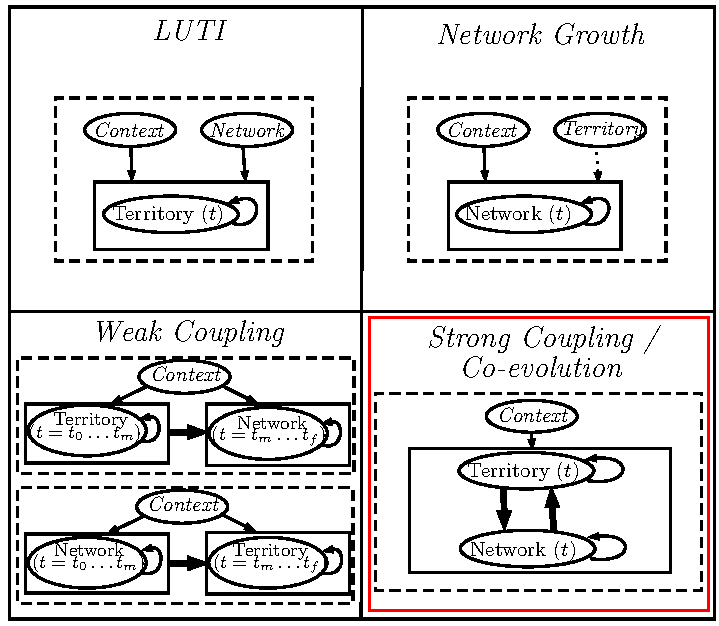
\includegraphics[width=\linewidth]{Figures/Modelography/coevolution}
\caption[Coupling types][Types de couplages]{Schematic representation of the distinction between different types of models coupling networks and territories}{\textbf{Représentation schématique de la distinction entre différents types de modèles couplant territoires et réseaux.} Les ontologies sont représentés par des ovales, les sous-modèles par les boîtes pleines, les modèles par les boîtes pointillées, les couplages par les flèches. Nous surlignons en rouge l'approche qui sera l'objectif final de notre travail.}
\label{fig:modelography:coevolution}
\end{figure}
%%%%%%%%%%%%%%%%%


Nous confondons échelle et portée pour ne pas rendre plus confus l'extraction. Nous différencions lorsque un élément n'a pas lieu d'être pour un modèle (NA) de lorsque celui-ci est mal défini par son auteur (\texttt{indef}). Nous ajoutons aux caractéristiques ci-dessus les variables suivantes issues automatiquement des classifications précédentes :

\begin{itemize}
\item Domaine de citation (le cas échéant)
\item Domaine sémantique
\item Interdisciplinarité
\item Interdisciplinarité au second ordre (le cas échéant, pour les références consistant en les deux premiers niveaux du réseau de citation)
\end{itemize}



Un ``bon choix'' de caractéristiques pour classer les modèles est un peu le problème du choix des \emph{features} en apprentissage statistique : si on est en supervisé, c'est à dire qu'on veut obtenir une bonne prédiction de classe fixée a priori (ou une bonne modularité de la classification obtenue par rapport à la classification fixée), on pourra sélectionner les caractéristiques optimisant cette prédiction. On discriminera ainsi les modèles que l'on connait et que l'on juge différents. Si l'on veut extraire une structure endogène sans a priori (classification non supervisée), la question est différente. Nous procéderons pour cela en second temps à une technique de regression permettant d'éviter l'overfitting et faire de la selection de caractéristique (Forêts aléatoires).


summary statistics ; correlations.


\paragraph{Classical Regressions}{Régressions classiques}

Nous commençons par étudier brièvement l'influence de divers facteurs sur les caractéristiques des modèles.



\paragraph{Random Forest Regressions}{Régressions par Forêts Aléatoires}




\paragraph{Unsupervised learning}{Classification non-supervisée}

\comment[JR]{également tenter une classif endogène des modèles : selon les caractéristiques récupérées.}




%%%%%%%%%%%%%%%%%%%%
\subsection{Discussion}{Discussion}


\paragraph{Further Developments}{Développements}

\bpar{
Further work may consist in the production of an automatic synthesis of this meta-analysis, from a modular modeling point of view, combined with a refined purpose and scale classification. Modular modeling consists in the integration of heterogeneous processes and implementation of processes in order to extract the set of mechanisms giving the best fit to empirical data~\cite{cottineau2015incremental}. We can thus classify models described here according to their building bricks in terms of processes implemented and thus identify possible coupling potentialities.
}{
Un développement possible pourrait consister en la mise en place d'une approche automatique à cette meta-analyse, du point de vue de la modélisation modulaire, combiné avec une classification du but et de l'échelle. La modélisation modulaire consiste en l'intégration de processus hétérogènes et d'implémentation de ces processus dans le but d'extraire les mécanismes donnant la meilleure proximité à des faits stylisés empiriques ou à des données~\cite{cottineau2015incremental}. L'idée serait de pouvoir extraire automatiquement la structure modulaire des modèles existants, à partir des textes complets comme proposé en~\ref{sec:quantepistemo}, afin de classifier ces briques de manière endogène et identifier des couplages potentiels pour des nouveaux modèles.
}



\paragraph{Lessons for Modeling}{Leçons pour la modélisation}









\stars



